%----------------------------------------------------------------------------------------
%	PACKAGES AND OTHER DOCUMENT CONFIGURATIONS
%----------------------------------------------------------------------------------------
\documentclass[a4paper,twoside,12pt]{article}
\usepackage{a4wide,graphicx,fancyhdr,amsmath,amssymb}
\usepackage[top = 25mm,bottom=25mm,left=25mm,right=25mm]{geometry}
\usepackage[usenames,dvipsnames]{color}
\usepackage{wrapfig}
\usepackage{todonotes}
\usepackage{float}

%\usepackage{pdfpages}
% Test if repo works.

%\usepackage{multicol}

\date{}	%default date null to make it not appear twice in titlepage




%---------------------------------------------------------------------------------------
%	MACRO'S AND DEFINITIONS
%---------------------------------------------------------------------------------------

\setlength\headheight{20pt}
%\addtolength\topmargin{-10pt}
%\addtolength\footskip{20pt}

\newcommand{\HRule}{\rule{\linewidth}{0.5mm}}
\newcommand{\N}{\mathbb{N}}
\newcommand{\ch}{\mathcal{CH}}
\newcommand{\solution}[1]{\noindent{\bf Solution to Exercise #1:}}

\def\Version#1{\def\version{#1}}
\newcommand{\revision}{\noindent{Revision: \version}}
\renewcommand\contentsname{Table of Contents}
\setlength\parindent{0pt}
\setlength{\parskip}{1em}


\author{Team-Beta}

%----------------------------------------------------------------------------------------
%	TITLE DEFINITION
%----------------------------------------------------------------------------------------
\title{
		\center
		%----------------------------------------------------------------------------------------
		%	HEADING
		%----------------------------------------------------------------------------------------
		\textsc{\LARGE Eindhoven University of Technology}\\[1.5cm] % Name of your university/college
		\textsc{\Large DZC20 Design for Games \& Play II - }%\\[0.5cm] % Major heading such as course name
		\textsc{\large Team Beta}\\[0.5cm] % Minor heading such as course title
		%----------------------------------------------------------------------------------------
		%	MAIN TITLE
		%---------------------------------------------------------------------------------------
		\HRule \\[0.4cm]
		{ \huge \bfseries Serious Games - Final Report: \\ \vspace{1em}Jumper}\\[0.4cm] % Title of your document
		\HRule \\[1.5cm]
		%----------------------------------------------------------------------------------------
		%	AUTHOR
		%----------------------------------------------------------------------------------------
		\begin{minipage}{0.4\textwidth}
		\begin{flushleft} \large
		\emph{Authors:}\\
        Team Beta
		\end{flushleft}
		\end{minipage}
        ~
		\begin{minipage}{0.4\textwidth}
		\begin{flushright} \large
		\emph{Course responsible lecturer:} \\
		prof.dr. B.A.M. Schouten BA
		\end{flushright}
		\end{minipage}\\[1cm]
		{\large Last modified: \today}\\ % Date
		{\normalsize \revision}\\[1cm]
        %--------------------------------------------------------------------------------------
        % Group members table
        %--------------------------------------------------------------------------------------
        {\normalsize \hspace*{-5em} \begin{tabular}{|l|l|l|l|}
        \hline
         \textbf{ Team Member} &  \textbf{Role} &\textbf{E-mail address} & \textbf{Student ID} \\ \hline
          Jeroen van Hoof & Coding/art/sound& j.m.a.p.v.hoof@student.tue.nl & 0778486 \\ \hline
          Kevin Cleijne & Art Assets, Evaluation
          &k.c.g.a.cleijne@student.tue.nl & 0779007 \\ \hline
          Pieter Kokx & Lead Programmer & p.a.kokx@student.tue.nl & 0747517 \\ \hline
          Joep Klein Teeselink & Programmer & j.klein.teeselink@student.tue.nl & 0816396 \\ \hline
          Twan van Schijndel & Level and Story Design & t.v.schijndel@student.tue.nl & 0857767 \\ \hline
          \hline
        \end{tabular}}\\[1cm] %---------------------------------------------------------------------------------------
		%	LOGO SECTION
		%---------------------------------------------------------------------------------------
		
\includegraphics[scale=0.2]{logo.png}%\\[2cm] % Include a department/university logo - this will require the 		graphicx package
		%----------------------------------------------------------------------------------------
		\vfill % Fill the rest of the page with whitespace
}


%---------------------------------------------------------------------------------------
%	HEADNOTE AND FOOTNOTE
%---------------------------------------------------------------------------------------

\fancypagestyle{plain}{
\fancyhf{}

\fancyhead[LE]{\sffamily\bfseries\large Last modified: \today}
\fancyhead[LO]{\sffamily\bfseries\large Final Report: Serious Game}
\fancyhead[RE]{\sffamily\bfseries\large DZC20 Design for Games \& Play II}

\fancyfoot[RO]{\sffamily\bfseries\large Team Beta}
\fancyfoot[LE]{\sffamily\bfseries\large University of Technology Eindhoven}
\fancyfoot[RE]{\sffamily\bfseries\thepage}
\fancyfoot[LO]{\sffamily\bfseries\thepage}

\renewcommand{\headrulewidth}{0pt}
\renewcommand{\footrulewidth}{0pt}
}

\pagestyle{fancy}{
\fancyhf{}

%\fancyhead[LE]{\sffamily\bfseries\large Last modified: \today}
\fancyhead[LO]{\sffamily\bfseries\large Serious Game Design}
\fancyhead[RE]{\sffamily\bfseries\large DZC20 Design for Games \& Play II}

\fancyfoot[RO]{\sffamily\bfseries\large Team Beta}
\fancyfoot[LE]{\sffamily\bfseries\large University of Technology Eindhoven}
\fancyfoot[RE]{\sffamily\bfseries\thepage}
\fancyfoot[LO]{\sffamily\bfseries\thepage}

\renewcommand{\headrulewidth}{1pt}
\renewcommand{\footrulewidth}{0pt}
}

\begin{document}
%--------------------------------BEGIN Version--------------------------------
\Version{0.5}
%--------------------------------END Version--------------------------------

\maketitle

%if having a titlepage add the % in front of the next lines:

\thispagestyle{empty}
\newpage
%----------------------------------------------------------------
%----------------------------------------------------------------
%if having a table of contents remove the % in front of the following lines:
\pagestyle{empty}{\tableofcontents}
\newpage
%----------------------------------------------------------------
\pagestyle{fancy}
\section*{Introduction}
This report covers the process of the creation of a Serious Game designed for programming courses. The goal is to provide an insight into the design philosophies, choices made and hurdles overcome. We will first discuss the basic premise of the game. Afterwards we provide an overview of the design concepts, realization and finally conclusions with individual evaluations.

\begin{figure}[H]
\centering

\includegraphics[scale=1]{teamlogo}
\end{figure}


\section{Goal}
Our objective is to create a serious game designed to pique interest in Computer Science. We intend to do so with a sandbox-like puzzle platformer that teaches you the basics of a programming language through its mechanics.

The game itself must be fulfilling to play, providing a reward system as you go which consists of acquiring new abilities in the form of programming commands, unfolding the story and encountering new and interesting locations with more difficult puzzle elements. When the player finishes the game, he should have a basic understanding of a programming structure.


\subsection{Target Audience}
Our game is intended for people who are looking for an introduction into programming and are interested in following a Computer Science education.
The demographic is aimed at high school students who wish to follow a computer science education. They need not have a background in programming, but should they do they will progress trough the game quicker and arrive at more challenging stages more quickly, increasing the level of programming required as levels progress.

\subsection{Team Introduction}
\begin{figure}[H]
\centering
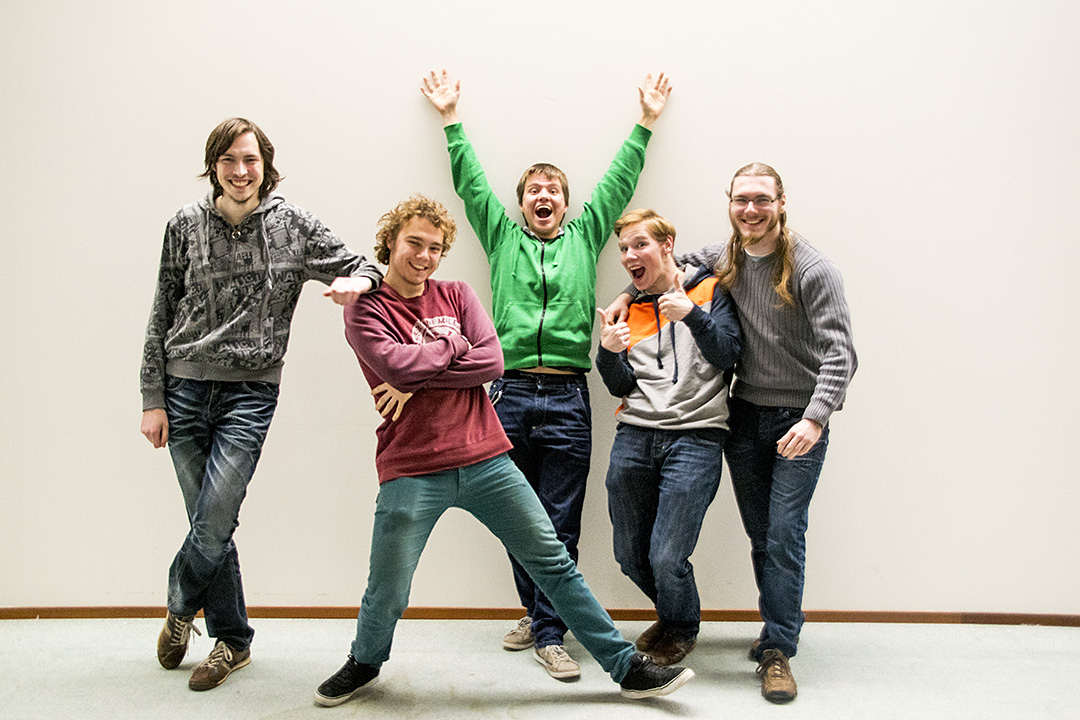
\includegraphics[scale=0.4]{group}
\caption{Jeroen, Joep, Pieter, Twan, Kevin}
\end{figure}
Our team consists of 5 members

\begin{itemize}
\item Jeroen van Hoof is a Web Science student (4th year).
\item Pieter Kokx is a Computer Science student (5th year).
\item Twan van Schijndel is Web Science Student (2nd year).
\item Joep Klein Teeselink is a Psychology and Technology student (3rd year).
\item Kevin Cleijne is a Software Science student (3rd year).
\end{itemize}


\subsection{Role Distinction and Allocation}
We define the following roles necessary for our game: \\

\textbf{Art Design - Jeroen van Hoof, Kevin Cleijne} \\
The art design makes up the aestetics of the game. We uphold a single standard art style to keep the looks consistant. We wish to create our own assets to make the game unique. The Phaser game induced two extra challenges: making blocks tile nice and using spritesheets for animation. We used Inkscape for most of the assets, GIMP for tileable blocks, since that worked better in GIMP and Adobe Photoshop/Illustrator because Kevin prefered to work with those tools.\\

\textbf{Programming - Jeroen van Hoof, Pieter Kokx, Joep Klein Teeselink} \\
The game is built using the Phaser HTML5 game framework, a HTML5 engine used to create web-based games using WebGL/Canvas. Phaser ships with support for arcade physics, a preloader to load all assets before the game starts, support for animation with spritesheets, particles and some other handy things. Phaser allowed us to focus more on the game itself, while exploiting its features.\\

Because we wrote our code in Javascript, everyone with a modern browser can play our game by just visiting the web page. There is no need to download or install anything. Since JavaScript is very popular, it is very easy for interested parties (including our own team members) to contribute to the project.\\

We started off building a library so that we could later on put the levels together really easy. For example, the function createPlatform() tiles a block-sprite, tests for collision and plays the land/walk-sound on collision with some additional screenshake and particles if the robot collides with it.\\

A next challenge was to let the player interact with parts of code. The way we coded the game, made it possible to access the entire game via the command line. We have however made a list of functions that are more easily accessible so that we could use it in the game. And we used jQuery-terminal so that the player can interact with this object via an in-game terminal.\\

\textbf{Level Design - Twan van Schijndel} \\
Our game is a puzzle platformer and as such level design is critical. The levels need to be created in a way that keeps the challenging yet not too complicated, pacing is key. \\

\textbf{Sound - Jeroen van Hoof}\\
For our sound, we mainly used the Youtube Audio library, and Audacity to cut in the sounds to take the best part out for use in our game. The jumping sound comes from Mario, the 'hey' when typing help() comes from the Legend of Zelda, and the jetpack sound comes from some Star Wars video. For every platform we used different walking and landing sounds, so that you really 'feel' the material of the platform or object.\\

\textbf{Evaluation and Testing - Everyone}
A game has to be iterated upon and bugfixed during its creation. It is imperative to detect bugs early and fix them, upholding structure and design principles. Any irregularities, defects and bad ideas need to be caught and adapted in order to make a functional and enjoyable game.\\

\subsection{Setup}

For our development setup we used a GitHub Repository, allowing every member to work on the project at once. Conflicting files can be easily combined to a single file and every modification is clearly documented via the GitHub client. Additions and alterations are traceable and revertible with ease.

The game design concepts are documented in Google Drive - we documented images and ideas while brainstorming. This allows us to look back on our work and recall discussions and ideas, saving the result of brainstorm sessions for later.
\todo{add images}


The communication channels we used were primarily via WhatsApp and Facebook. These let us schedule appointments for when to come together and attend people to ideas and progression. We also utilized the GitHub issue section to flag problems and assign them to team members to fix.

\section{Game Concept}
We aim to create a puzzle platformer that teaches players a programming language as they play it. We keep the player entertained with interesting environments, story progression and nice visual/auditive effects. We want to allow the player to experiment with the coding language, providing them with a 'common' solution as well as other ways to go about the problem. When the player gets a good grasp of the coding language he could find special methods that enables him in finding a new solution altogether, rather than following the standard procedures of puzzle solving. We want the player to think about his programming abilities and exploit them in the game to figure out new and interesting ways of solving the situation at hand.
as the player progresses he encounters new and interesting levels, acquires new programming skills while advancing the story.

We use a basic flat design art style that keeps things simple and clear, allowing for easy distinction between background visuals and foreground objects/platforms. For easy access to the game we opted to create it in a HTML game engine called Phaser, which allows us to deploy the game online, no installation necessary.

\subsection{Story}

\begin{figure}[H]
\centering

\includegraphics[scale=1.5]{jumper}
\caption{The protagonist: Jumper}
\end{figure}

Ultimately the game aims to teach the basics of programming - so what better protagonist than a robot?
Jumper is a matrass-tester on the run from his overseers from the matrass factory. He breaks lose from his testing-chamber/prison and ventures out into the world. Luckily for him his jumping skills are quire adapt and he can easily traverse the treacherous areas outside of the facility. However that he soon finds that this is not enough and he has to rely on his new-found knowledge of the World-Programming installed upon him in his escape of the factory. Why is it that he can program certain objects? Where can he find more knowledge about this power? Who else is stuck in the factory? Who released him? Follow Jumper's quest and find out.


\subsection{Gameplay Elements}
%\includegraphics[width=14cm]{ss2.png}
The game allows for manipulation of the world around you using a programming terminal. Certain objects can be interacted with and re-programmed to move around, become solid or unsolid, activate or deactivate, ...
the interactions increase as you progress, making things more interesting and difficult as you go. To not overwhelm the player we have introduced a help() command that provides you with insight into what is going on and what you can do, how it works and provide hints to a solution. You can think of the help command as a sort of catalogue explaining the workings of a particular programming function/method. The game requires some precision jumps and puzzle solving (via programming) which keeps things fresh. You can approach the problem in many different ways. A player might be inclined to traverse the level, solving obstacles as he encounters them, or they may sit back and think about the level - program/solve it and then finally traversing the puzzle in one swoop. They can even think of ways to reach the end by using hidden functions at their disposal, which they can find by experimenting and knowing the programming language better. Picking up hints to these 'secret' methods throughout the game.

\subsection{Level Design}

Puzzle platformers require good level design to be fun to play. The levels need to be challenging and incorporate the different programming abilities via obstacles that should be logical elements and not feel very out of place. To achieve a good level we adhered to a standard of keeping objects as a power of 2, generally picking 32px by 32px for a standard platform, having the player character at 32x64. By adhering to this standard we can precisely place objects and platforms for the different levels.
Special attention is given to the introduction/tutorial level(s),aiming to
create a connection between the player and the playable character. The
tutorial levels introduce new programming mechanics - the objective of what
the player needs to do to progress is clearly visible, it is up to him to find
out exactly how the command works - turning to the help function when in
doubt, as well as tips displayed in the level. We wished to make the solution
not very <do this> like but instead attempted to blend the solution in the
background, having the player observe behaviour occurring in the game and
learning from that.
\todo{tracks/machine idea discussion here if implemented}.

\begin{figure}[H]
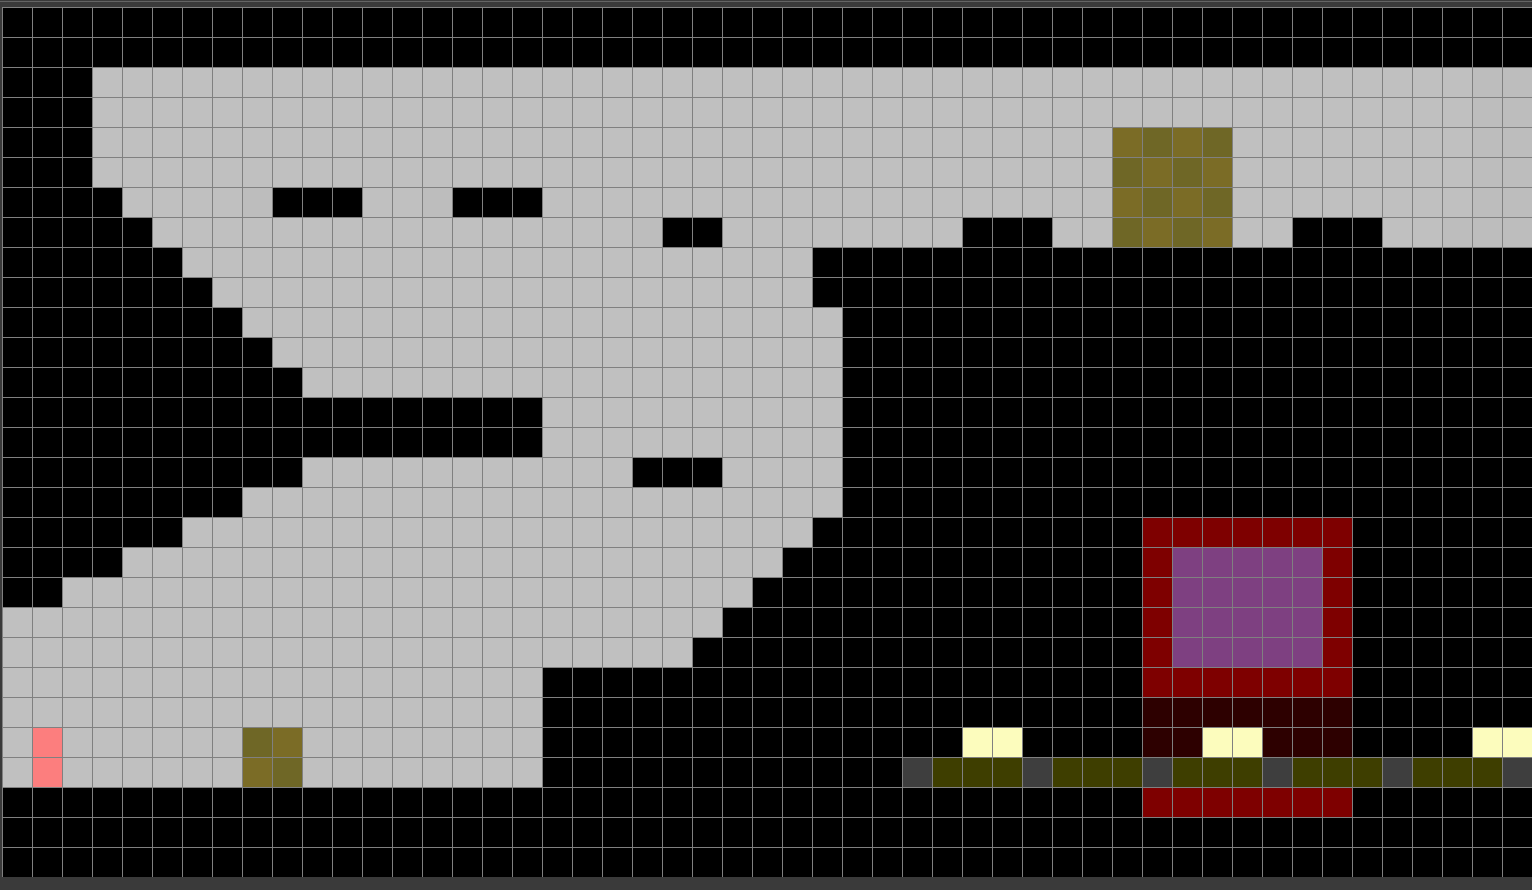
\includegraphics[scale=0.5]{level.png}
\caption{tutorial concept}
\end{figure}

\section{Realization}
Now that we have the game concepts in place, we need to actually create a game.
We opt for a HTML game that can be deployed online for easy access. Platformers are not as resouce intensive which allows for this approach. Levels can be loaded fast and there is practically no downtime. This approach allows us more flexibiltiy, utilizing a HTML engine Phaser, as well as some CSS and Javascript to further enhance the game.
%Phaser/game structure
\subsection{Structure Realization}

\todo{need a back-end guy to talk about Phaser canvas and game structure a
    bit.}


\subsection{Programming Habits}
\todo{talk about standards employed}

\subsection{Game Interaction}
The interactions the player has with the game are basic platforming with a jump combined with the puzzle aspect, solvable using the command terminal used to manipulate objects. The terminal allows for programming of game objects, calling upon readily made functions (and some hidden ones to allow for experimentation) that can change the world so that you may advance the level. Since we do not require players to have a programming background, we have to supply them with the know-how of these manipulations. To assist in this we need to have a tutorial for each of these new programming aspects. After such a tutorial we need to provide a codex to re-evaluate the just learned mechanic. We do this by means of a help() function. Upon calling the help while trying a manipulation we provide an insight into its workings and further explain the usage. To further assist the player in doing some tedious tasks we incorporated a click mechanic that will pre-write the object name whenever the player clicks on a manipulatable object in the game world, giving it a while border implying it is selected. This click auto-fills the terminal and makes it ready for manipulation.

To improve the gameplay and clarity of the game, we have plenty of visual and audible queues, giving a clear indication when something goes wrong or right, as well as an error report in the terminal - telling you what went wrong. We use screenshake for a more tactile experience while playing the game. Falling on objects has actual weight to it due to the shake, which increases the faster you crash into something. Each object has a landing sound attached to it - changing the effect depending on what type of surface you interact with.

Animated objects allow for a lively world that is interesting to look at. Some of them incorporate a mechanic, such as a bouncing matrass and conveyor belts, others are just visual effects designed to fluff up the world. 


\subsection{Level Creation}
The levels have been designed on paper prior to implementation to the game. The conceptual drawings follow the 32px by 32px rule of a single block, allowing for a good scalable representation of the level and accurate platform distancing, to be traversed by Jumper. Conceptual levels introduced new mechanics which we then incorporated as programming functions for the game, such as having obstacles dissipate and become unsolid or having objects stand in the way of your level progression. These ideas were drawn and incorporated into a playable level, then created as functions and realized in the game for the player to solve.

\begin{figure}[H]
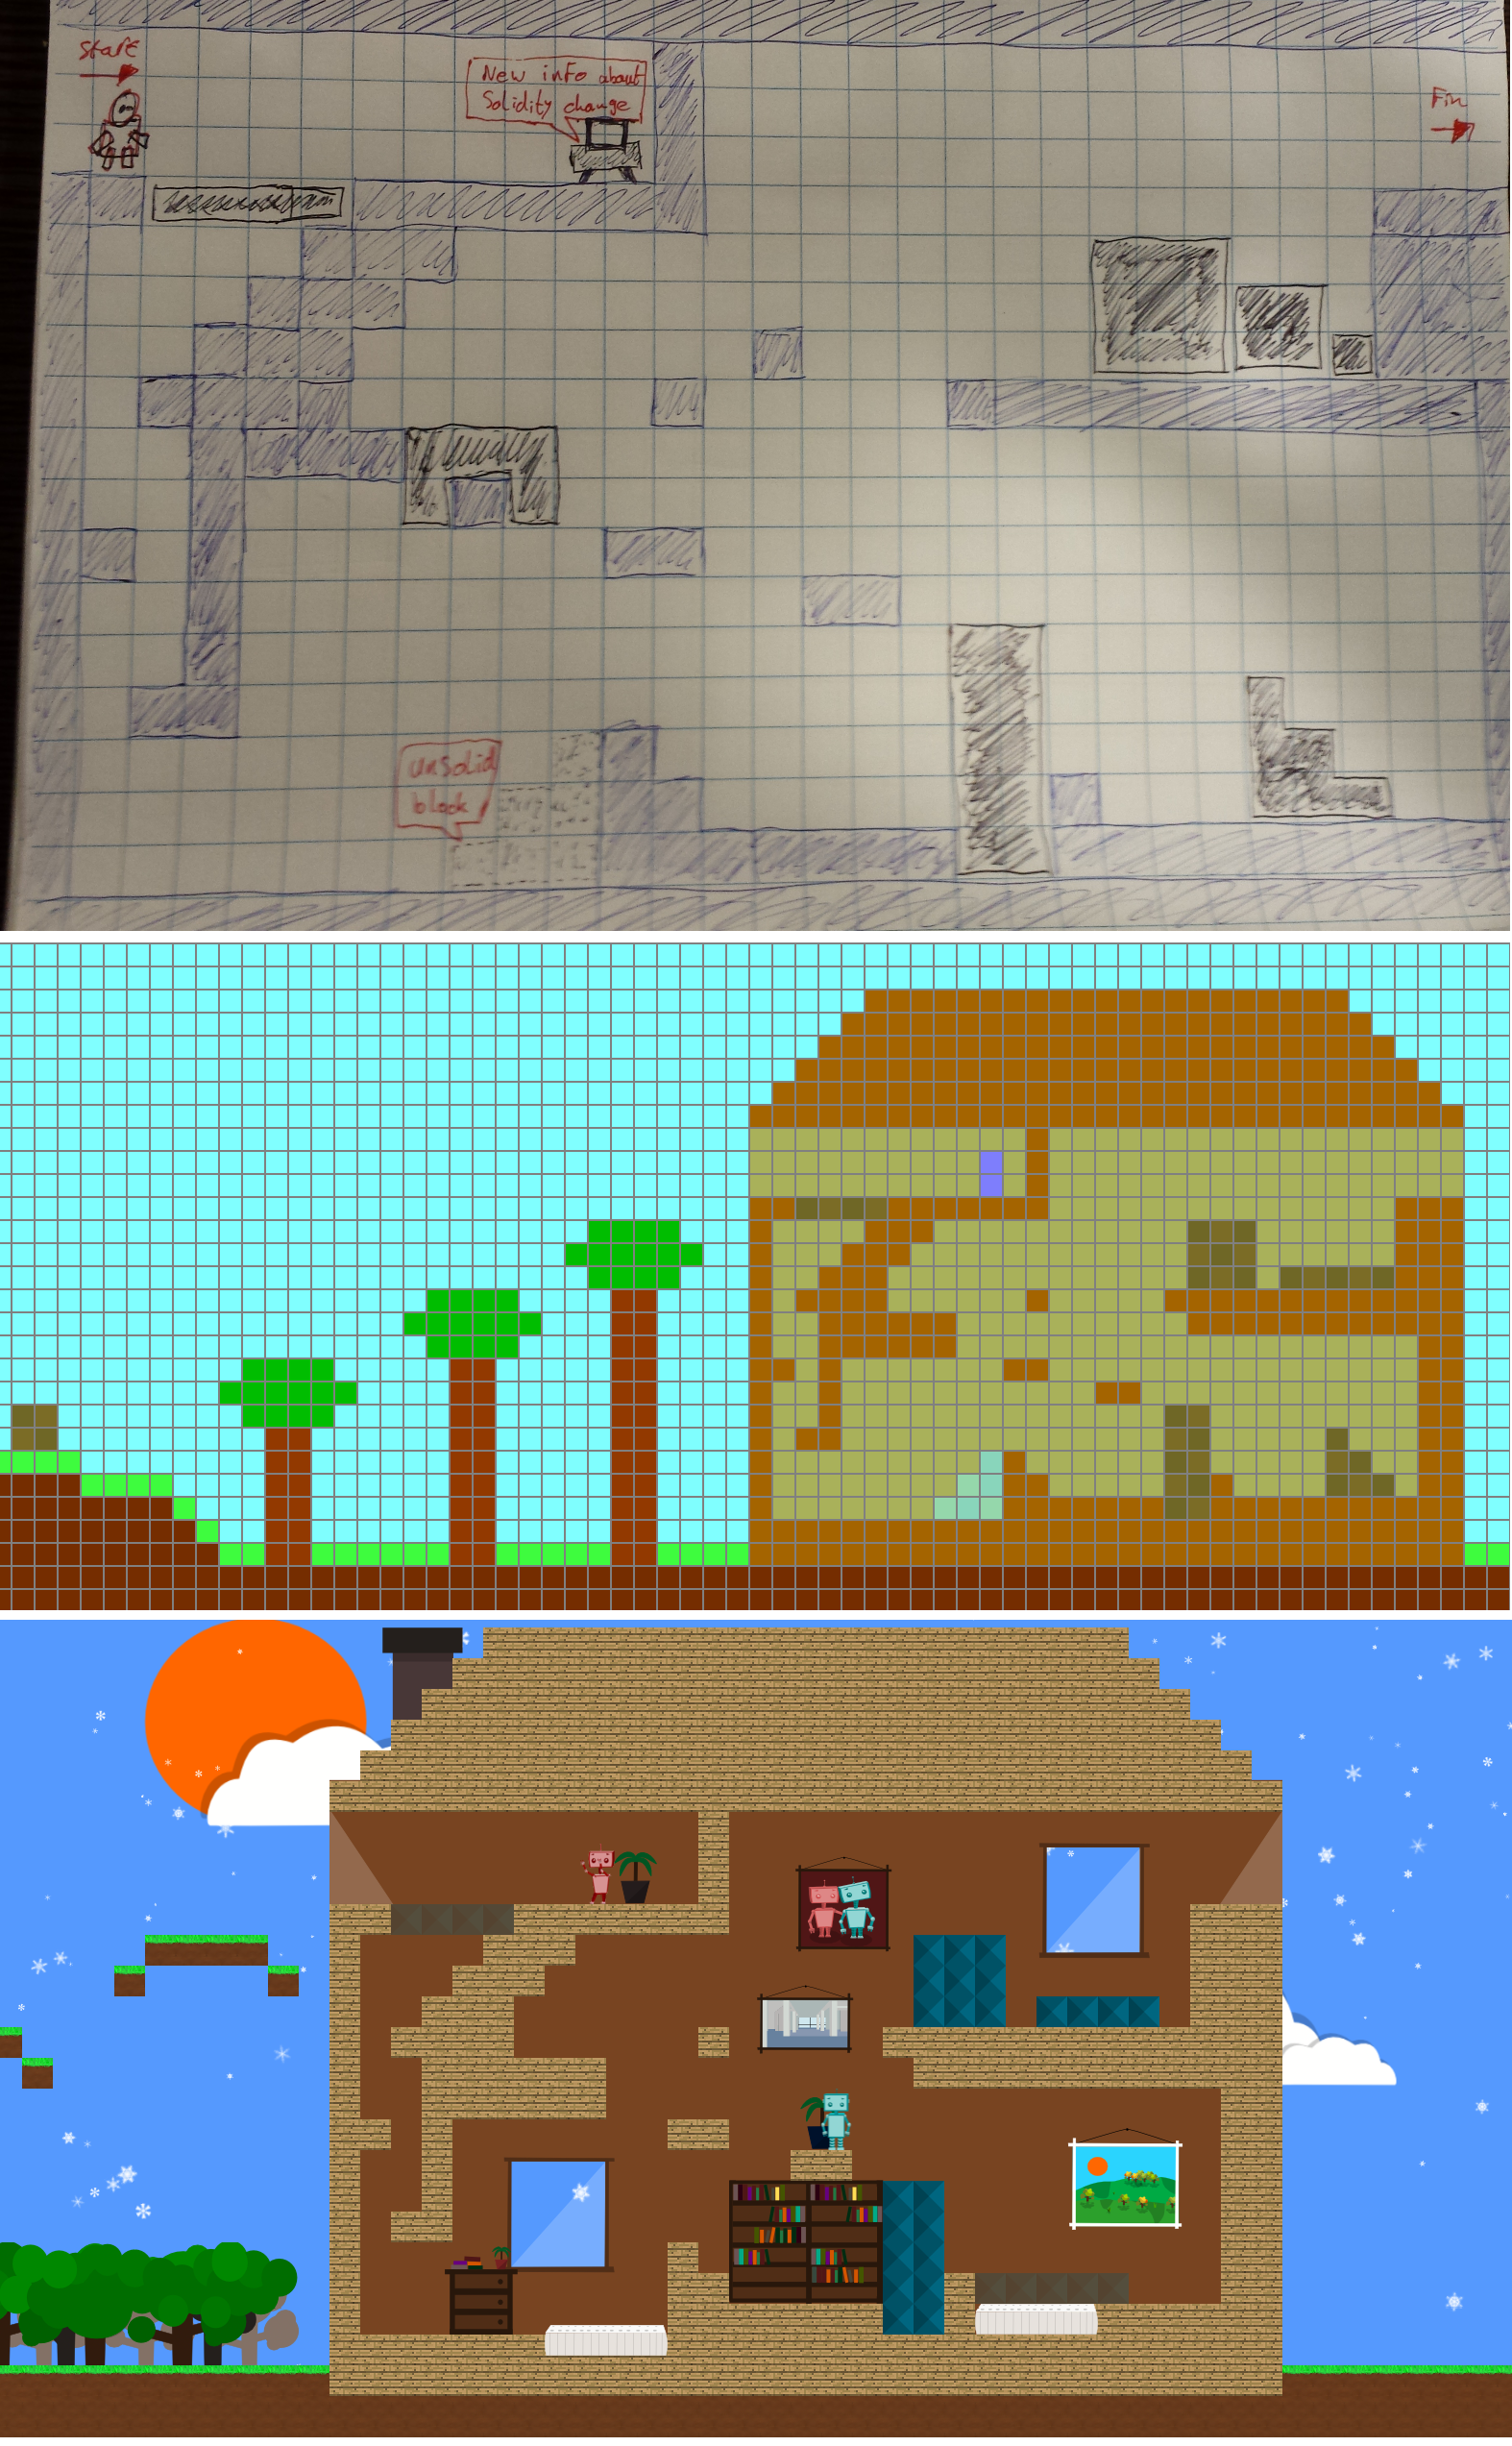
\includegraphics[scale=0.3]{levelSketchAndDesign.png}
\caption{The process of level creation for level 3}
\end{figure}

%art 
\subsection{Art Creation}
The art assets were made by 2 members, and as such it was difficult to adhere to a single style, we used assets that were made in a way that it was not clearly obvious that two people created them. The style we used is called Flat Design. Even though it appears basic, there are subtle effects in play that require some effort to realized. As such we had to scrap a lot of assets, removing them entirely or having to heavily modify them to fit to the standard. The assets themselves are vector drawings, able to scale up and down without resolution loss. This allows us to
change the scale of assets on the asset itself rather than use Phaser to manipulate scaling. As long as the assets adhered to the ratio rules we set, they would fit perfectly into the canvas. Even if this did not work out it was easy to change the scale on the asset itself, them being vectors instead of rasterized images.

\section{Iteration}
We started out creating the basic structure of the game, setting up a UML
diagram which we adhered to. We had to do some renaming to make everything
more logical when dealing with the code, having 2 different classes called
Game is ambiguous and has been resolved by renaming one to Main.
\\
\begin{figure}[H]
  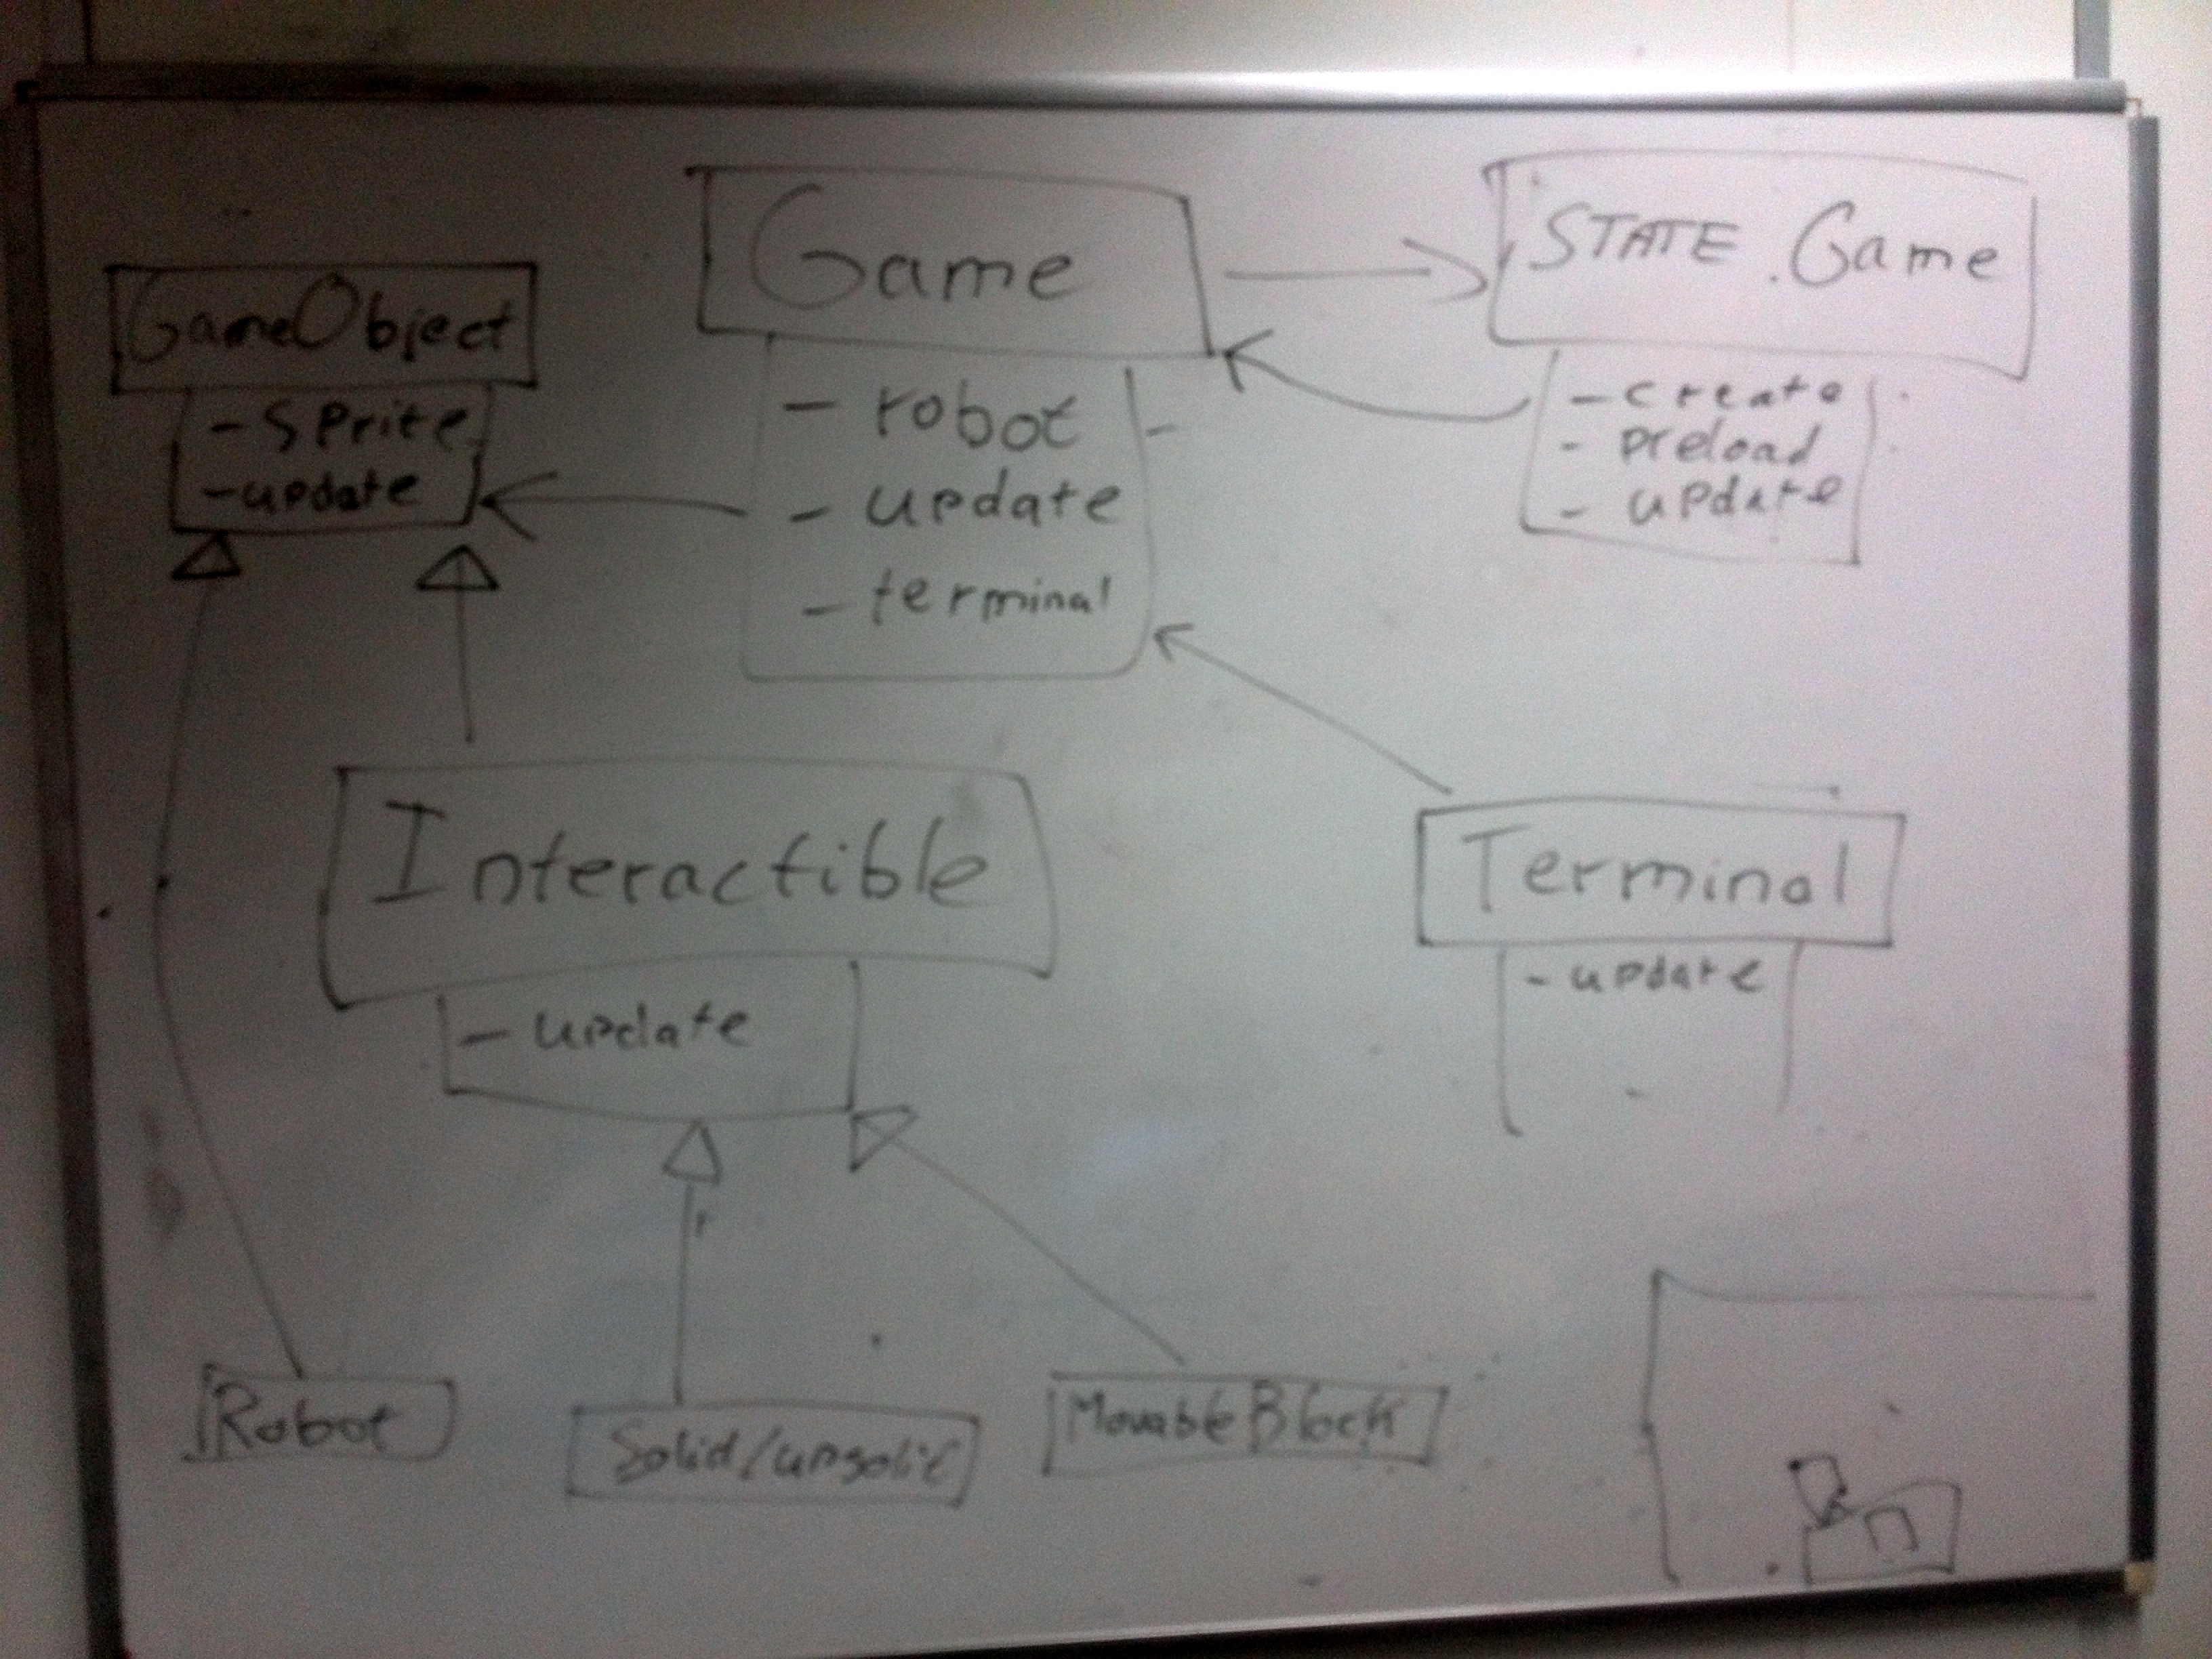
\includegraphics[width=1\textwidth]{API}
  \caption{API structure} 
\end{figure}

Many assets have been revised and updated to fit the style we opted for, different scales have been made and are readily present in the repository, allowing for easy adaptation where necessary. Others have been discarded or heavily manipulated.
\begin{figure}[H]
  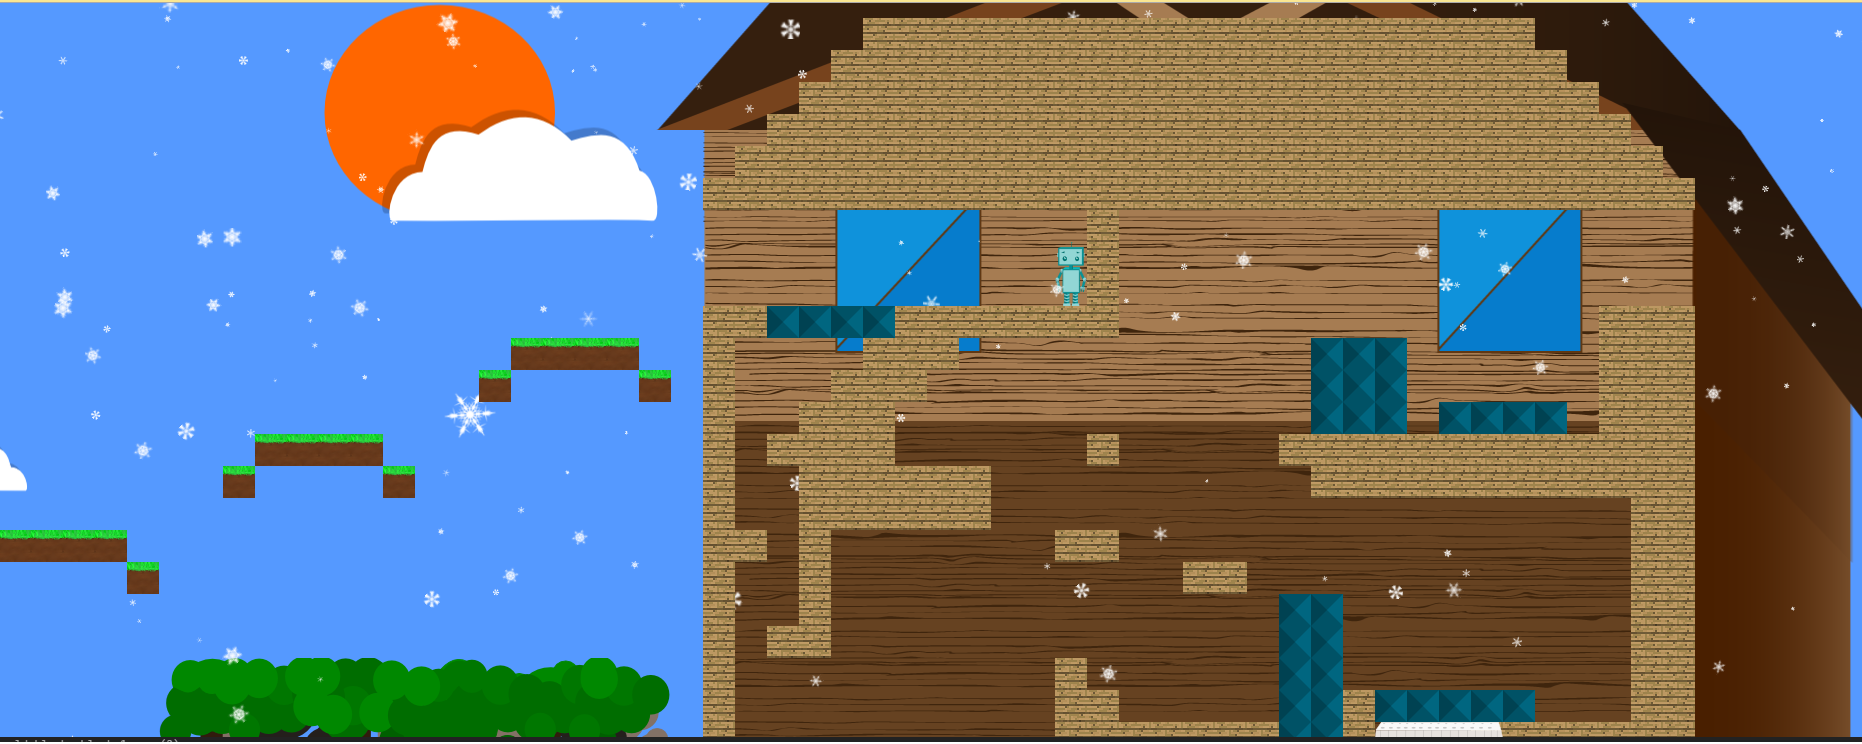
\includegraphics[width=1\textwidth]{house_1}
  \caption{House: first iteration}
\end{figure}
\begin{figure}[H]
  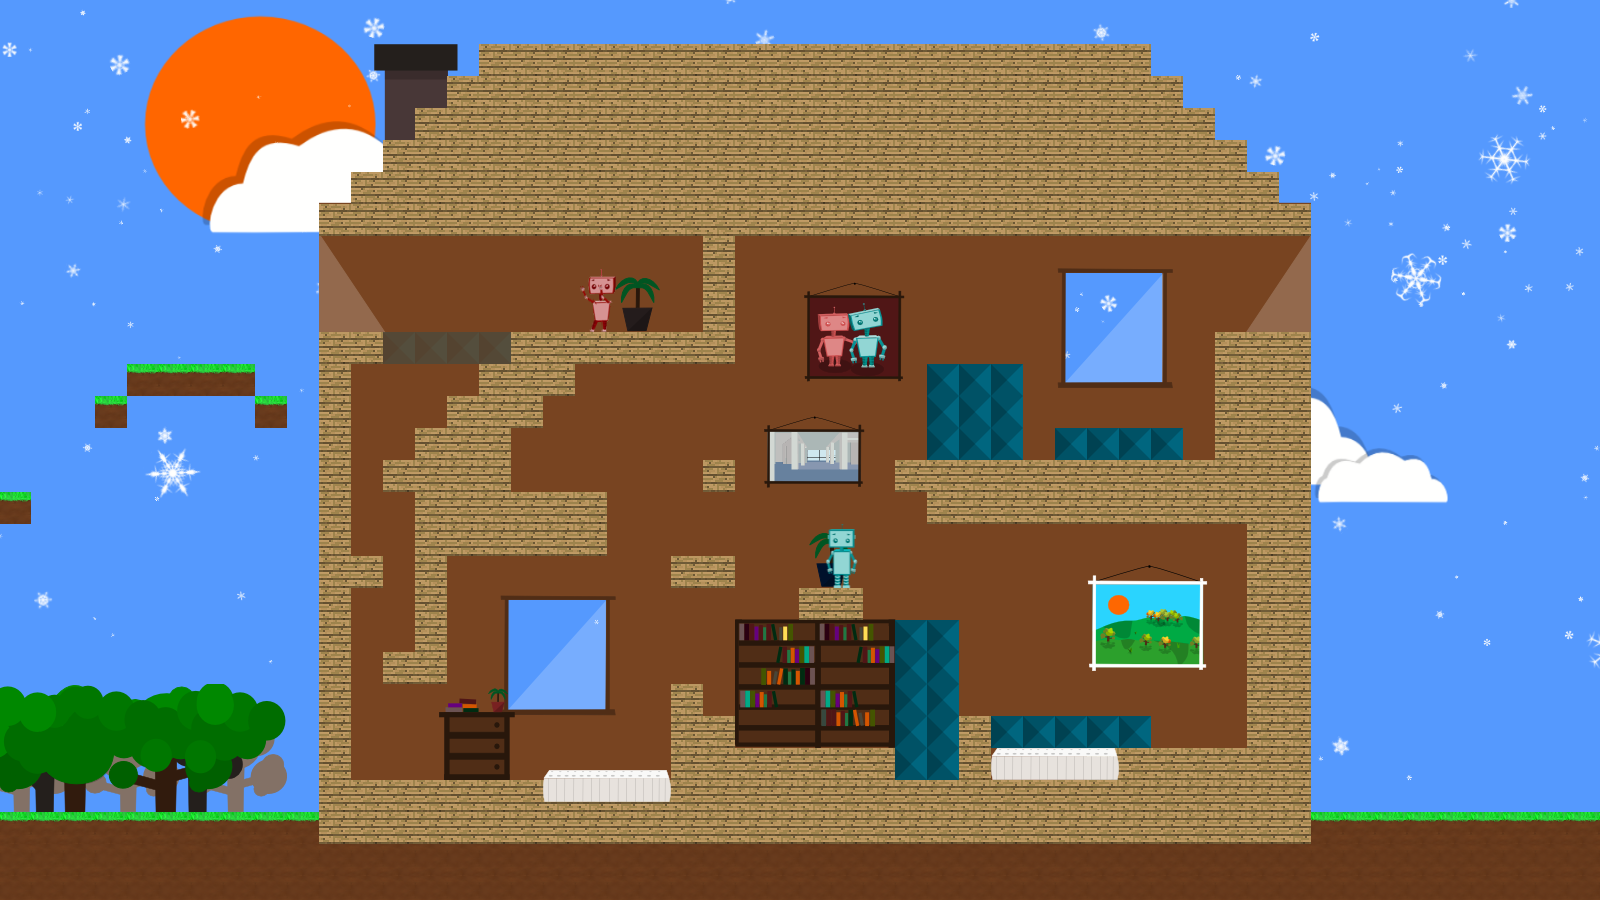
\includegraphics[width=1\textwidth]{house_2}
  \caption{House: last iteration} 
\end{figure}

We had several ideas for the Interface - first opting for floating text boxes
when clicking on an object to list it's name, properties and affected methods.
We opted for a terminal help function instead to avoid cluttering the game
with boxes and avoid having many clicks. The focus is to 'write/code' your way
trough the game, not click. Further we discussed some clarity changes - where
each specific manipulation such as solid/unsolid() or move() would be visually
queued by having those objects appear in a certain color only.
\todo{is this still the case or is it ambigous now?}
We looked to color-code parts of the terminal input to make it clearer for the player, ultimately we had to scrap that in favour of a more robust terminal. 
\begin{figure}[H]
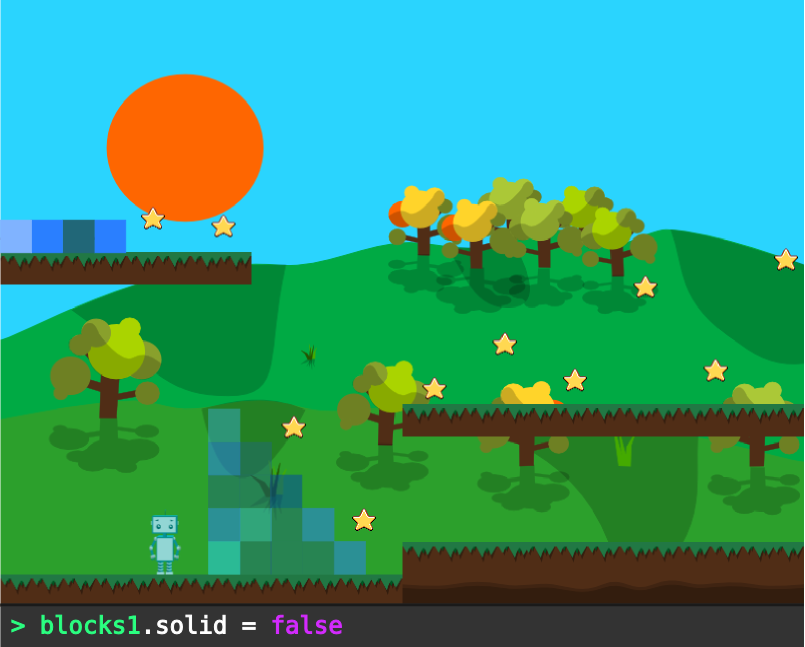
\includegraphics[scale=0.6]{terminal_example.png} 
\caption{terminal}
\end{figure}

Our initial level was made up of a single defined area, later we introduced a camera motion that allows us to make bigger levels that scrolls with the player. This allowed for more complex and larger levels.
The story progression should have a logical ordering for the levels, creating a factory level where you first become acquainted with Jumper, traversing the factory to escape into the wide world. These world locations should follow some logical sequence. We wanted to make the areas diverse and interesting so the idea was to make a neon-city progression, where you would visit the outskirts with defect robots, the inner city full of life at night-time and visit the center with a mall and disco. We instead decided to create a progression that first explains the mechanics more so we introduced the goal 'get to the TU/e' for Jumper, where would learn more about his abilities.
\begin{figure}[H]
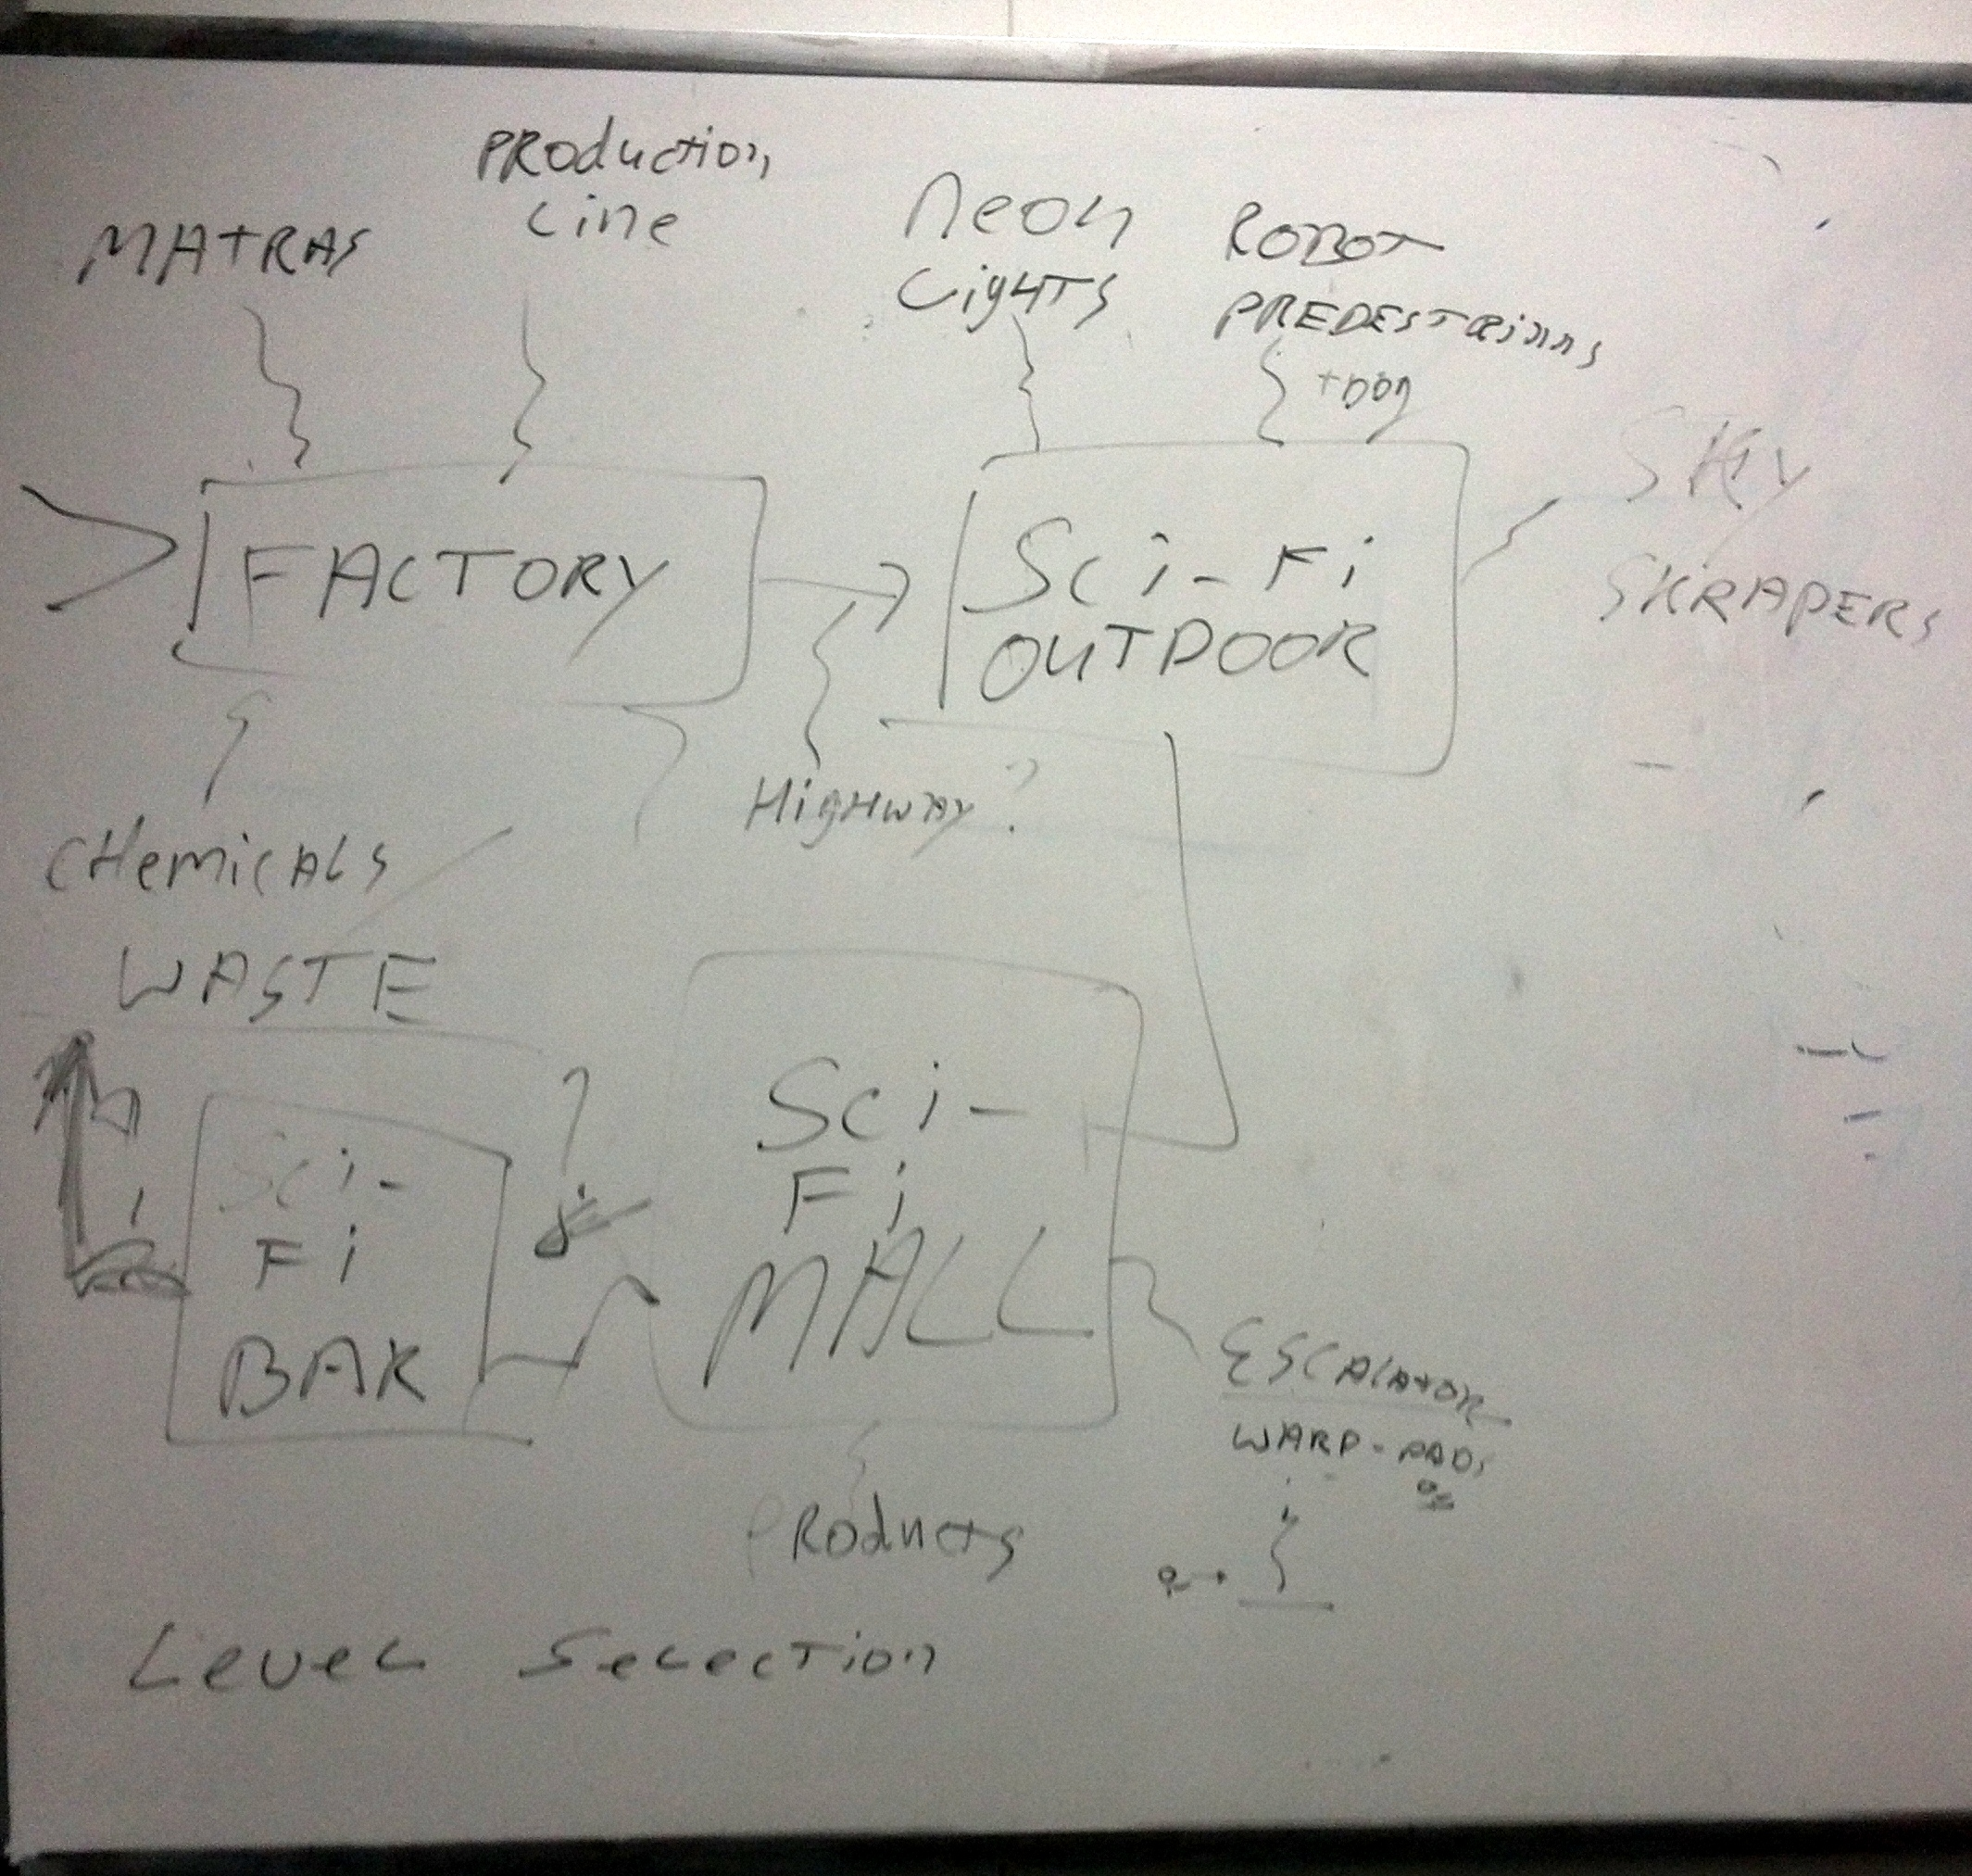
\includegraphics[scale=0.2]{locations}
\caption{level progression}
\end{figure}
When we started user testing, we found out that the players did not really like the game. First of all, they did not understand why they had to type commands, but after we explained to them that it was a game to learn programming, they understood. What we found out to be the biggest problem, was that users did not really like to type. After a while they would get bored. We already reduced this by letting users click on an object and insert part of the required code in the terminal, but they still had to type the entire method themselves. So, we created a menu that would automatically execute commands. The problem with that was that players did not learn to type their commands out, and the distance to actual programming became to big. We solved this by gradually extending the list of commands that could automatically be executed from the menu each time the user learned and practiced the command enough. And we put in an extra 'select' option that would insert first part of the code for all commands that still required typing. 

Another problem was that users did not know what to do in the intro level. They had to type help(), then go through the block that became unsolid and follow the hallway. But it was not clear that the block changed, so we did a few things to fix this issue. First, we made the difference between the solid and unsolid state more distinct by making the block more transparent in the unsolid state. Next, we also added a transition sound every time the block changed state. We also updated the help() function so that it said "that block blocking the exit" instead of "that block over there". And finally, we added blinking arrows, that basically just yelled "Go there!".\\

The fun thing, but also the most challenging thing, about building our game was, that if we changed one little thing, it would affect the entire gameplay and all strategies of solving a level, and even the entire initial level design could be needed to be redesigned. The gap between a challenging game and an overpowered block or robot was very small. For example, if we had added a resize-feature that lets you resize blocks, you could just resize blocks to get over them instead of making them unsolid, or resize them instead of moving them to the right spot so that you could jump on a higher platform... or imagine what happened if we allowed the blocks to float in the air. One other exampple is the world.robot.jetpack(true) function that would give the robot a jetpack with which it could just fly to the end of the level without solving things. We had to degrade the jetpack by removing the unlimited height you could go to, and then it was still overpowered, so we decided to let it just in as an easter egg.\\

We made all interactable objects the same form and color, just like in Mario, to make a very clear distinction between game objects that could not be programmed, and the ones that can. First, our blue blocks could only teleport. There was no gravity or collision detection, and they just could be placed everywhere you want them to be. So instead of solving puzzles, you could just select all blocks and move them to wherever you want. Next, we added some basic gravity, collision with platforms, game objects and other blue blocks. And changed the teleport to a change in velocity (.moveRight(100) would move the block to the right with a speed of 100 pixels/s). Later, we changed that to a task-queue that would just move with a preset velocity and check if the block has moved so many tiles to the right and then stop.\\

Somehow, the blocks pushed you throught the underneath ground if they fell upon you. This was not easily fixed, I mean, we could just let it stay on the head of the robot or something, but instead of fixing it, we transformed it into a feature, by adding in a level where you could exploit this 'feature' to your advantage. I think this fit our game well, since we wanted to allow people to be able to hack or break the game.\\


\section{Evaluation}

%----------------------------------------------------------------------------

\subsection{Individual report - members motivations and reflections}

\subsubsection{Kevin Cleijne}

I enjoyed the course as a whole but felt that we had too similair backgrounds to really structure the roles. The game we made was a puzzle platformer which does not require a 
storyline as much as something like a point-and-click, which was my previous role. I decided to work on art assets and help out Jeroen but it proved difficult to adhere to the standards of flat design, as I had no experience with vector drawing. During the project I tried to help out in different areas, mostly making basic assets and doing the documentation of the design principles for Google Drive and the final report. Looking back I feel that I should have lead the project more, allowing proper focus and clear, crisp ideas/objectives for us. A lot of work proved unusable because of communication errors and unacknowledged requirements for assets that I made, requiring heavy modification or even removal of them. For the next project we really need to have a crystal clear communication line where everyone knows exactly what to expect from another. I will need to have a look at what is at our disposal with GitHub, see if we can get these requirements clearly visible. We need to set deadlines and expectations for designs we wish to include so that we have plenty of time to incorporate it properly.
I need to communicate better and ask exactly what is required of me so that the effort is not lost, which is a shame.

\subsubsection{Jeroen van Hoof}

I liked the idea to use Phaser. The previous course we wrote our own browser-based point-and-click engine with HTML, JavaScript, PHP, and CSS. And now we could upgrade to a browser-based platformer game with pure JavaScript. So, our group name upgraded as well from Team Alpha to Team Beta. Who knows, Team Gamma next? It could make up for some nice puns... Gamma, that I say! It is nice that we acquired Pieter from the Pixel-evolution group who already used Phaser, now we can combine forces!\\

In the first course, I had tossed the idea to use GitHub to speed up our development. Unfortunately, nobody really had experience with GitHub, so we had used Dropbox/Filezilla and a host Joep had somewhere left. This was kind of ugly, but at least everyone understood it. But with the introduction of Pieter in our group, we could push GitHub trough, after some boggle here and there ;). I was very happy about this.\\

I was very impressed by the Vlambeer presentation back in the first part of the course. So, right off from the start, I said "Screenshake!". I did not care what this screenshake would be used for, as long as we would have screenshake somewhere. It is a little feature that makes the game much more lively, but because it is so little, it is also easily overlooked. Since there are no guns or enemies in our game, I ended up using it for the landing of the robot: the harder it landed, the longer the screen shaked. Together with some particle effects and a land sound, it really feels like you land on something hard. The best thing is that mattresses do not cause a screenshake, which makes them feel very soft and pleasant to jump on, next to the cold rumbling steel conveyor belts in the intro level. Also, because every block has a different matching walk and land effect, you really get to 'feel' the game.\\

I learned quite a few new things this quartile. I learned a new HTML5 game framework, some advanced JavaScript, a bit more about git, editors, to make spritesheets for animation, making tile-able blocks, and more. But most importantly, how to make a funny serious game.\\

\subsubsection{Pieter Kokx}

I joined a team that had already worked together in the previous Design for
Games and Play course. That made it a bit difficult in the beginning to get
started, because the rest of the team already had a history together. It
easily became clear that I was the more seasoned programmer in the team, so I
moved myself into the role of lead programmer rather quickly. Since I had a
great experience with the Phaser framework in the previous course, I proposed
to use it during this course as well. And I'm glad we did, because it made the
game easy to play on all computers.

In the beginning, I set out to make sure that we have a good setup of the
source code. Looking back at it, I'm glad that we took our time to do that.
Because of our solid codebase, it was possible for us to move very quickly
when we needed to. In the last two weeks, it was very easy to add new levels,
and to implement new features.

I also introduced the team to the notion of using git and GitHub as version
control tools. Instead of using a file-sharing tool like Dropbox, which tends
to generate a lot of conflicted copies when multiple people work on the same
file, these versioning tools allow you to properly merge these problems when
the arise.

During this project I think we, as a team, helped each other to make a great
product. I really like the game that we created. I also like the solid
codebase which we have. If we would continue to work on the project, I know
that we can easily add a lot more features to the game.


%\includegraphics[width=14cm]{ss9.png}
\subsubsection{Joep Klein Teeselink}

The games for design and play courses have been a joyful and interesting ride for me so far. Both projects I did with this group have been very fun and educative to me. This project was different from the last one in a way where in the previous course I had a more leading role (especially when it came down to the code) and thus, was much more involved on how things were going at any given moment. In this course we had a new member joining our team (Pieter) who is a much more experienced programmer than me. He took over the lead programmer role and showed us a great way to make use of a browser-based engine. The brainstorm sessions in the beginning were really inspiring as we had a new stream of thoughts which made our ideas swirve in a different direction than the last project. Pieter gave us some new insight on possibilites we didn't think of and thanks to this we started using Phaser. It was then up to us as a team to come up with a good concept and some basic goals the game should have. I felt like we all had a good contribution in this part of the project, and I was happy with the outcome. After we started working on the actual game it was difficult for me to prove worthy as someone else took over the lead programmer role. I felt like I had to take it easy and let one person work out the engine of the game before things got messy. After we had a working core and we were ready to implement our creative aspects which would make this game the game it became I really started coming loose and tried to help out wherever I could to make sure we would end up with something we could be proud on. We would devide roles and set issues in GitHub so everyone would always be up-to-date with what had to be fixed/added in the game. I felt like our meetings were good and connected this group as a whole. The amount of time we spend together figuring out bugs and finding improvements really improved my teamwork skill. Whenever we had a new issue or a idea everyone's opinion was taken seriously and handled with care. This made working together a really beneficial aspect of our group.

\subsubsection{Twan van Schijndel}

I really liked this course of Design for Game and play II. It was very interesting to learn about the psychology in gaming. I especially liked the project we had. Even more so than the project of Design for Game and Play I. I felt much more usefull for my team this time and I really, really liked designing the game and its levels. I had to think about the story of the game that would engage the player, what programmable powers would be fun for our type of game and how the buildup in each level should be. I also had to think about what might be fun mechanics for our game that were actually possible with the amount of time and knowledge we had. I've created about six level sketches on paper and worked out 4 of them as coloured pictures with the right dimensions on my laptop. After that I created the levels in the game and added and added an extra one. Eventually the 3 best levels that were possible with the mechanics we had made it into the final game and I am very proud of that. I think they are a good fit for our game and that they are fun to play, challenging enough and slowly teach the player more about their powers.\\
The teamwork in this group was also of high quality. My knowledge of programming and the programs we used to work on the project was fairly limited. But there was always someone that was willing to help me out.\\
I am really proud of our game and all the work we put into making it.

\section{Appendix}
\todo{THIS}


\end{document}
